% 2009 年湖北卷文科第 18 题：四棱锥 S-ABCD。
% 来源 PDF：普通高考/2009/2009湖北文.pdf，SHA-256 f60ba7a5a2fef3449fba9474fa973c616aa52a15926b3a97f0dda6b909f4c861。
% 原页：第 2 页第 1 栏上部，书页码 526。
% 重绘依据：底面 ABCD 为正方形，SD⊥底面，故 SD 画成竖直线并落到底面顶点 D 上；
%   D 在锥体内部，SD、DA、DC、AC 与 E 到 A、C 的连线均被遮挡，画虚线；
%   SA、SB、SC、AB、BC 为可见棱，画实线。E 为 SD 上一点（DE=λa）。
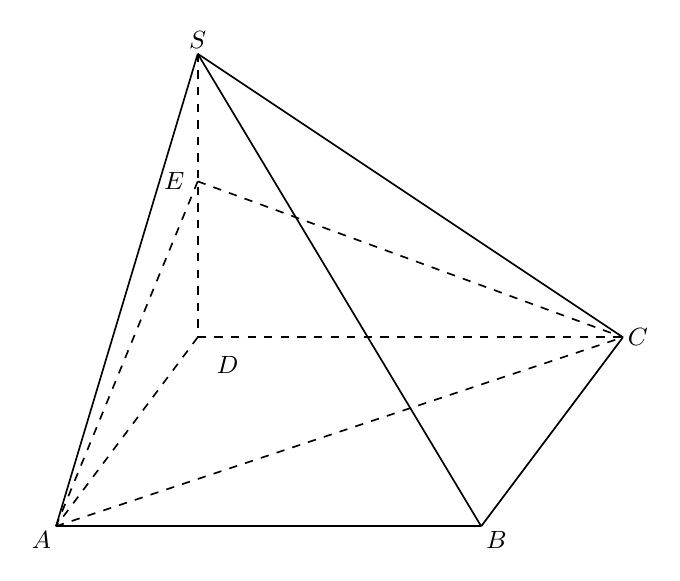
\begin{tikzpicture}[semithick, every node/.style={inner sep=1.5pt, font=\small}]
  \coordinate (A) at (0.2,1.2);
  \coordinate (B) at (5.6,1.2);
  \coordinate (C) at (7.4,3.6);
  \coordinate (D) at (2.0,3.6);
  \coordinate (S) at (2.0,7.2);
  \coordinate (E) at (2.0,5.58);

  % 可见棱
  \draw (S) -- (A);
  \draw (S) -- (B);
  \draw (S) -- (C);
  \draw (A) -- (B);
  \draw (B) -- (C);

  % 被遮挡的棱
  \draw[dashed] (S) -- (D);
  \draw[dashed] (D) -- (A);
  \draw[dashed] (D) -- (C);
  \draw[dashed] (A) -- (C);
  \draw[dashed] (E) -- (A);
  \draw[dashed] (E) -- (C);

  % 标签
  \node[above] at (S) {$S$};
  \node[left=3pt] at (E) {$E$};
  \node[below right=5pt] at (D) {$D$};
  \node[below left] at (A) {$A$};
  \node[below right] at (B) {$B$};
  \node[right] at (C) {$C$};
\end{tikzpicture}
